\graphicspath{{./main/2_introduction/figures/}}

\chapter{Introduction}
\label{chap:intro}

Every single organism in an ecosystem has the property to have a life-form. Humans, as many of the other species organisms, are part of the biological evolution. Darwin states in~\citep{darwin1859} that all species of organisms arise and develop through the natural selection of small, inherited variations that increase the individual's ability to compete, survive, and reproduce. In order to fulfill the mention abilities, as living organisms we might need to perform a large subset of actions that will allow us to survive in our environment. Those actions can vary depending on each individual and can go from being able to communicate, grasp objects, or move from one place to another. However, in order to perform many of the mentioned actions we need to use our perception system so that we can gather and interpret our sensory information. The human perception system can be extremely complex and composed by several layers of sensory cells that respond to a specific type of physical stimulus that typically will be processed by our brains to finally perform specific actions.

One of the main purposes for using the human perception system is to reconstruct our environment which is very necessary to create an internal representation of everything that surrounds us that will help us at the time to plan and execute the above-mentioned set of actions. In this work we are going to focus more on how the human visual perception system works and how much related is to the study of the computation and information, also known as Computer Science. In concrete, we are going study the problem of Scene Reconstructions through different geometric Computer Vision techniques and how after analysing single or multiple set of images we can reconstruct the shape and appearance of real environments.

\section{Scene Reconstruction}

\begin{figure}[t!]
	\centering
	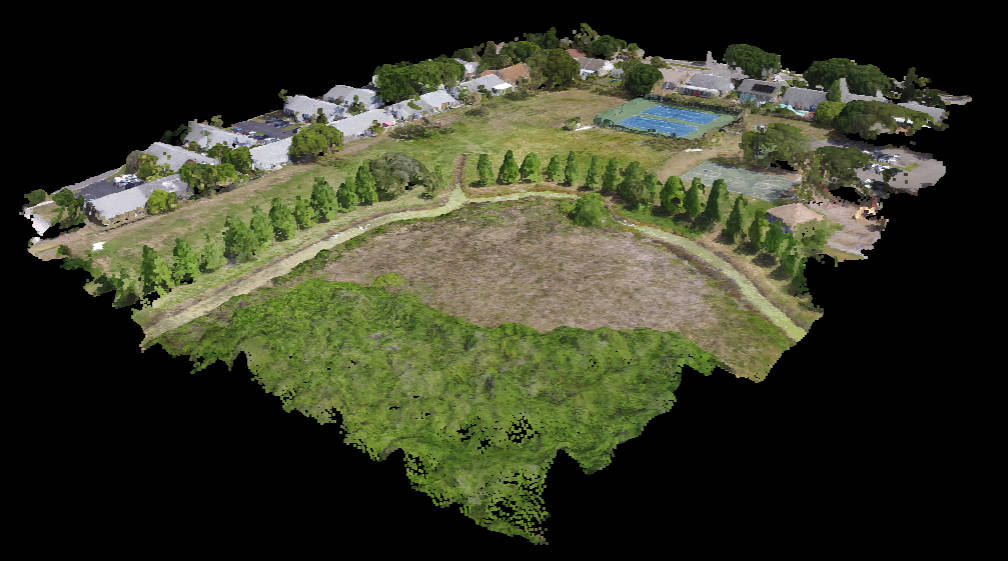
\includegraphics[width=\textwidth]{main/introduction/images/odm_reconstruction.jpg}
	\caption[Scene reconstruction problem]{\textbf{Scene reconstruction problem.} Reconstruction obtained using \textit{Open Drone Maps} an open source photogrammetry toolkit to process aerial imagery into maps and 3D models. As can be seen, the global structure of the scene is quite accurate after applying a st of combined geometric computer vision techniques. }
	\label{fig:intro_odm_reconstruction}
\end{figure}

In the previous section we referred to the term of Computer Vision, but \textbf{What it is Computer Vision and how related is to the task of reconstructing environments ?} To answer that question, we can describe first Computer Vision as a sub-field of Computer Science that tries to mimic the human visual system using computers in order to extract and analyse high-dimensional data from digital images or videos from the real world. Computer Vision is an interdisciplinary scientific field related to artificial systems and sometimes referred as, or part of the so known term Artificial Intelligence (AI) that works after extracting information from any kind of images. The type of images can vary depending on the scope of the application and can take many different forms such as single monocular images, video sequences, images from multiple cameras or multi-dimensional data from 3D scanners or medical scanning devices. Besides the types of images that can be acquired, the entire field can be divided into many sub-domains including event detection, video tracking, object recognition, 3D pose estimation, learning, indexing, motion estimation, visual servoing, 3D scene modeling, image restoration or scene reconstruction, which is the main topic that we will cover during in this thesis.

As we described in the previous section, as humans we have the inherited ability to learn to create abstract representations of the environment that we are surrounded and which will help us to perform later complex actions. In our modern era, where everything is automated, an open question is - \textbf{How can we make computers to reconstruct environments or scenes seamless as we humans do ?} The answer to that question is combining the human knowledge with the use of classical and subsequently advanced Geometric Computer Vision Techniques. In the field of Computer Vision, Scene reconstruction can be described as the process of creating a virtual representation of a real world entity from data obtained from different sensors such as images or scans.

There is a lot of literature around how to perform Scene Reconstruction in Computer Vision Techniques using as a main resource images. Scene Reconstruction can be used in many fields such as Robotics, Medicine, Augmented reality, Archaeology, or 3D object recognition, among others. However, in order to solve the task will be very depending on the application and the type of sensors that will be used during the design of the setup. In order to introduce the problem of Scene Reconstruction we will split them in two main categories: \textbf{Local Features} and \textbf{Dense} methods, that later will be explained in more detail along this thesis with the proposed contributions for each of them.

In the early days of Computer Vision many of the proposed methods have been based on detecting features that are discriminative enough to solve a specific task. However, sometimes choosing the right features for an application can be a crucial decision that will affect the final performance of the method. The different types of features in Computer Vision and Image Processing can go from detecting edges, corners (or interest points), or blobs (regions of interest points). Every type of feature has its own pros and cons and as we mentioned each application may have different requirements that will make the researchers swing between one or a combination of different features.

\subsection{Local Features}

\begin{figure}[t!]
	\centering
    \begin{tabular}{c}
    	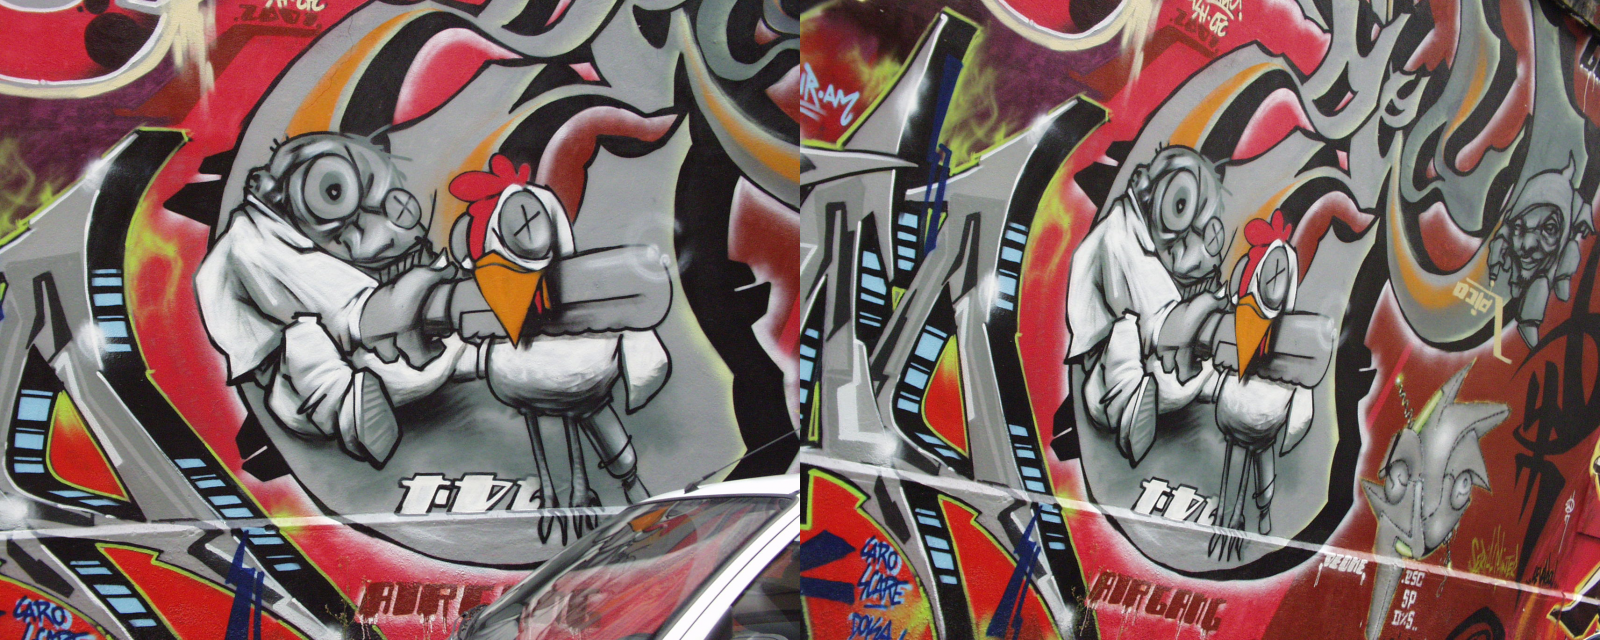
\includegraphics[width=\textwidth]{main/introduction/images/local_features_graffiti.png} \\
    	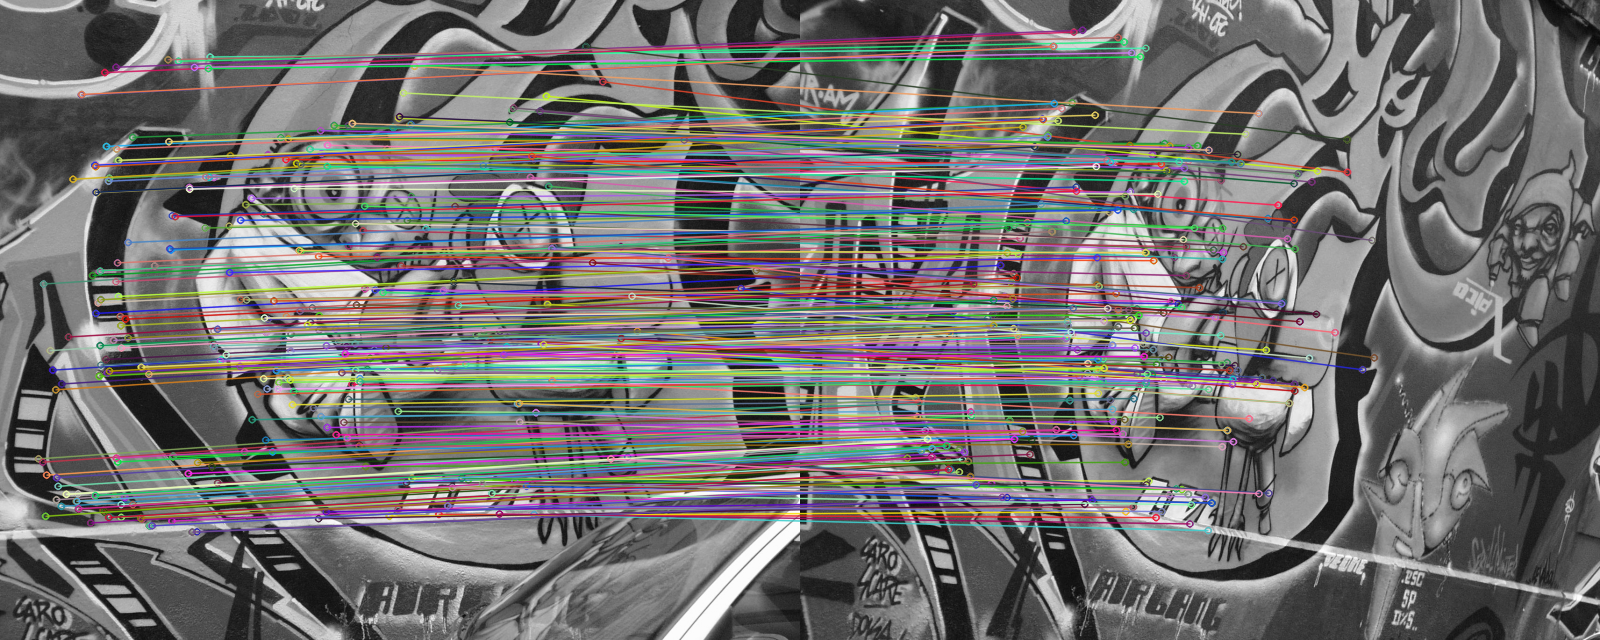
\includegraphics[width=\textwidth]{main/introduction/images/local_features_graffiti_matching.png}
    \end{tabular}
	\caption[Local features matching problem]{\textbf{Local features matching problem.} Row (a) shows images of two consecutive of dogs of the \emph{dhole} breed, while (b) shows dogs of the \emph{dingo} breed. As it can be seen, de differences in pose have more impact on the appearance than the breed. }
	\label{fig:fine_grained_dogs}
\end{figure}

In this thesis we will give a strong focus on the usage of local features in a scene reconstruction pipeline. However, in first place - \textbf{What is a local feature and what the advantage of using them?} As described in~\citep{tuytelaars2008local} a Local Feature can be described as an image pattern which differs from its intermediate neighborhood. Considering that the most common image properties are intensity, color and texture; Local Features can take different forms such as points, but also edgels or small image patches, that later will be converted into descriptors mapping the image properties that we just described. Local Features are a powerful tool that has been successfully used in different applications for instance edge detection in aerial images that often corresponds to roads; blob detection that can be used to identify impurities in some inspection task, etc. However, in our case we are more interested in the fact that Local Features can be really relevant as long their location can be determined accurately and stable over time. For this reason, are very useful in application such as matching or tracking and specially for camera calibration or 3D reconstruction. Since our interest will be the usage of Local Features for Scene Reconstruction pipelines using Geometric techniques, in the next paragraphs we will review its usage in a couple of applications.

One of the most popular problems where scene reconstruction takes an important role is in Robotic mapping, which typically is the task to create a map based on the information captured but the robot perception system. This problem can be also referred as Simultaneous Localization and Mapping or commonly known as SLAM, which using computational geometry, tries to construct and update a map of an unknown environment while simultaneously keep tracking the agent location withing it. The classical pipeline for solving SLAM problems based on input images, involves several intermediate steps that can be shared across many other applications. One those intermediate steps, and the one that we will focus more in this thesis, consists in extracting local information or also known as Local Features, from images that later combined with different geometric techniques can be used to compute either the agent location or for updating the map reconstruction.

Another popular problem which scene reconstruction appears to be an important key component is Structure from Motion (SfM). SfM can be described as the technique associated to the field of photogrammetry that tries to estimate a three dimensional representation from a two-dimensional image or a set of them based on the local motion between the different view information. The main principle for SfM is based on the motion parallax theory that using the difference between the displacement of the different views and from the depth information will be used to estimate an accurate 3D representation of the world around them. Finding the structure from motion it is directly related to stereo vision since in both cases it is needed to have a geometric relation between the different image views. This is another sub-problem in the classical pipeline, to find pixel correspondences that relates one pixel from one image to another, typically with sub-pixel precision. The process for finding correspondence is typically solved by extracting Local Features, and as we mentioned before, can be done using techniques with the same theory background that the ones used for solving visual SLAM problems.

\subsection{Dense methods}

Scene reconstruction cannot be only solved with sparse methods using local features as we described in the previous section. In traditional Computer Vision there is a lot of literature about using other type input data coming from different types of sensors such a stereo systems or depth cameras. Stereo systems are designed in a similar way as our perception system works. Based on two equidistant cameras, the goal is to produce a depth map that will map for every pixel the distance where the surface of an object is. To work with stereo systems has a lot of pros and cons, since its uses RGB cameras and usually in a calibrated setup which the baseline between the camera is known and helps a lot with the process to solve the depth. However, the use of RGB images can be a bit critical since they are a bit noisy in front of light changes and this might affect the final result of the depth maps.

Several works have been trying to solve stereo vision using classical methods [check for papers], or even recent ones that use CNN to feed the two images on the network to produce a depth map. Another, approach to compute depth maps is directly using Range imaging such as structured light or time-of-flight camera which are able to produce already very approximated depth maps. The information obtained from this type of cameras is very valuable for some applications such as in robotics since it solves part of the pipeline for finding the 3d representation of the environment. Range cameras are not the solution to this problem since they are also affected by different lighting conditions and can produce sometimes inaccurate results and artifacts in the predicted depth maps. Recent methods try to solve monocular depth estimation using CNN which produce very challenging results compared to classical methods.

The mentioned methods are usually computationally expensive in normal scenarios and almost impossible to use in real applications such as in robotics where other high level tasks depend on the perception algorithms. Cloth manipulation is one of the tasks that fully relies on a highly accurate estimation of the 3d shape of the object. Many robotics applications still use classical methods such as stereo systems, since RGB cameras are cheap and the algorithms used are very optimised for those platforms, or as described before others can use RGB-D cameras to avoid the cost of computing depth maps. The final goal for such applications is to get an reconstruction of the scene as much accurate as possible in order to determine different high level task, for example the planning for a the trajectory of a robot arm. It is common that when working with single or even stereo-cameras we suffer from a common problem in vision produced by the motion parallax which is the lack of information from a view or also known as occlusions. Having occluded parts in our observations can lead to several problems since we will loose precision later, making sometimes difficult to reason for the subsequent tasks. Some works try to solve this issue by providing more cameras to the system, also called mult-view stereo systems that by triangulation methods will complete the missing information. However, for some real applications having more cameras is not feasible, and a natural action would be to move the robot around to explore and complete the missing information from more observations. Another approach would be to provide extra information to the system such as the object mesh, that can be registered with local features and infer the camera pose respect to the object. Similar to other works, we propose later in thesis to synthesize views from an initial given pose of the robot in order minimize the effort of moving the robot around the object to manipulate.

% ----------------------------------------------------------------
\section{Thesis contributions} 

In this thesis, we analyze the different possible methods to perform scene reconstruction and focus in each of the parts of the pipeline, identifying the different issues, and propose solutions to them in each chapter:

\begin{itemize}
    \item In chapter 2, we analyze in detail the approach of detecting local features and computing descriptors from the extracted image patches for image matching and 3D reconstruction. In this chapter we will focus to show how traditional behave respect to CNN based methods and we compare with two proposed solutions - the first that improves a detector based on a geometry loss by learning CNN features, and the second, a shallow CNN that uses a Triplet loss to learn to produce local descriptors that improve previous state of the art methods for feature matching.
    
    \item In chapter 3, we will discuss about the use of mixed methods for classical and learned methods in the Computer Vision field. We provide an extensive review of different methods and applications from the software engineering perspective by proposing a new framework that combines classical Computer Vision with modern auto-differentiable methods. The chapter will also include several graphical and coding examples about how to use the proposed framework \textit{Kornia} in addition of a review for real applications where the framework is useful to.
    
    \item In chapter 4, we analyse methods to perform 3D reconstruction in a more dense manner using end to end systems based on CNN's. We also analyse the usage of such algorithms for robotics applications such as object manipulation where usually it is expensive to move the robot in order view the scene from different perspectives. For this reason, we propose a methods that can deal with novel view generation in similar scenarios for the case of cloth manipulation.
    
    
\end{itemize}

% ----------------------------------------------------------------
\section{First Published Appearances contributions}

This thesis follows the format of a publications which each chapter corresponded to an article or a subset of article in a journal or conference:

\begin{itemize}
    \item Chapter 2: Vassileios Balntas, \textbf{Edgar Riba}, Daniel Ponsa, and Krystian  Mikolajczyk. Learning local feature descriptors with triplets and shallow convolutional neural networks. In \textit{BMVC}, 2016.
    \item Chapter 2: Axel Barroso-Laguna, \textbf{Edgar Riba}, Daniel Ponsa, and Krystian Mikolajczyk. Key.Net: Keypoint Detection by Handcrafted and Learned CNN Filters. In \textit{ICCV}, 2019.
    \item Chapter 3: \textbf{Edgar Riba}, Dmytro Mishkin, Daniel Ponsa, Ethan Rublee, and Gary Bradski. Kornia: an Open Source Differentiable Computer Vision Library for PyTorch. In \textit{Winter Conference on Applications of Computer Vision (WACV)}, 2020.
    \item Chapter 3: \textbf{Edgar Riba}, Dmytro Mishkin, Jian Shi, Daniel Ponsa, Francesc Moreno-Noguer, and  Gary Bradski. A survey on Kornia: an Open Source Differentiable Computer Vision Library for PyTorch. In \textit{Journal of Engineering Applications of Artificial Intelligence} (under review).
    \item Chapter 3: Jian Shi, \textbf{Edgar Riba}, Dmytro Mishkin, and Francesc Moreno-Noguer. Differentiable Data Augmentation with Kornia. In \textit{Neurips 2020 Workshop: Workshop on differentiable computer vision, graphics, and physics applied to machine learning}, 2020.
    \item Chapter 4: \textbf{Edgar Riba}, Jordi Sanchez-Riera, Yurun Tian, Fan Zhang, Albert Pumarola, Yiannis Demiris, Krystian Mikolajczyk, and Francesc Moreno-Noguer. Novel View Synthesis of Depth Maps for Cloth Manipulation. In \textit{ICRA} 2021 (under review).
    \item Chapter 4: \textbf{Edgar Riba}, Jordi Sanchez-Riera, Albert Pumarola, Fan Zhang, Yurun Tian, Yiannis Demiris, Krystian Mikolajczyk, and Francesc Moreno-Noguer. Depth Map Synthesis for Deformable Clothes. In \textit{CVPR} 2021 (under review).
\end{itemize}